\documentclass[titlepage]{tufte-book}

\usepackage[runall=true]{pythontex}
\setpythontexworkingdir{<outputdir>}
\usepackage{environ}
\usepackage{morewrites}
\usepackage{amsthm}
\usepackage{amsmath}
\usepackage{amssymb}
\usepackage[pdftex]{graphicx}
\usepackage{epstopdf}
\usepackage{hyperref}
\usepackage{alltt}
\usepackage{listings}
\usepackage{array}
\usepackage{extarrows}
\usepackage{setspace}
\usepackage{tikz}
\usepackage{tikz-qtree}
\usetikzlibrary{calc}
\usetikzlibrary{positioning}
\usepackage{hyperref}
\usepackage{graphviz}
\usepackage{geometry}                % See geometry.pdf to learn the layout options. There are lots.
\usepackage{bashful}
\usepackage{microtype} % Improves character and word spacing
\usepackage{caption}

\usepackage{booktabs} % Better horizontal rules in tables

\setkeys{Gin}{width=\linewidth,totalheight=\textheight,keepaspectratio} % Improves figure scaling
\graphicspath{{figures/}}

\usepackage{fancyvrb} % Allows customization of verbatim environments
\fvset{fontsize=\normalsize} % The font size of all verbatim text can be changed here

\newcounter{problem}
\newcounter{total}
\newcommand{\step}[1]{{}
\vspace{4pt} \noindent {\bf \theproblem. }#1\addtocounter{problem}{1}}

\newcommand{\cut}[1]{}

\usepackage[tikz]{bclogo}
\usepackage{tikz}
\usetikzlibrary{calc}

\lstdefinestyle{BashInputStyle}{
  language=bash,
  basicstyle=\small\ttfamily,
  numberstyle=\tiny,
  showstringspaces=false,
  numbersep=3pt,
  otherkeywords={|, ;, ', ", *,>, <, *, &, `, $},
  alsoletter={:~_},
  columns=fullflexible,
  backgroundcolor=\color{yellow!20},
  linewidth=0.93\linewidth,
  xleftmargin=0.03\linewidth,
  keywordstyle=\color{blue},
  emph={ls, cat, head, tail, more, less, sort, uniq, kill java, grep, zip, unzip, tar, wc, cp, chmod,chown},
  emphstyle=\color{black}\bfseries,
    commentstyle=\color{gray}\slshape
    }

\newcommand{\chili}{\scalebox{.04}{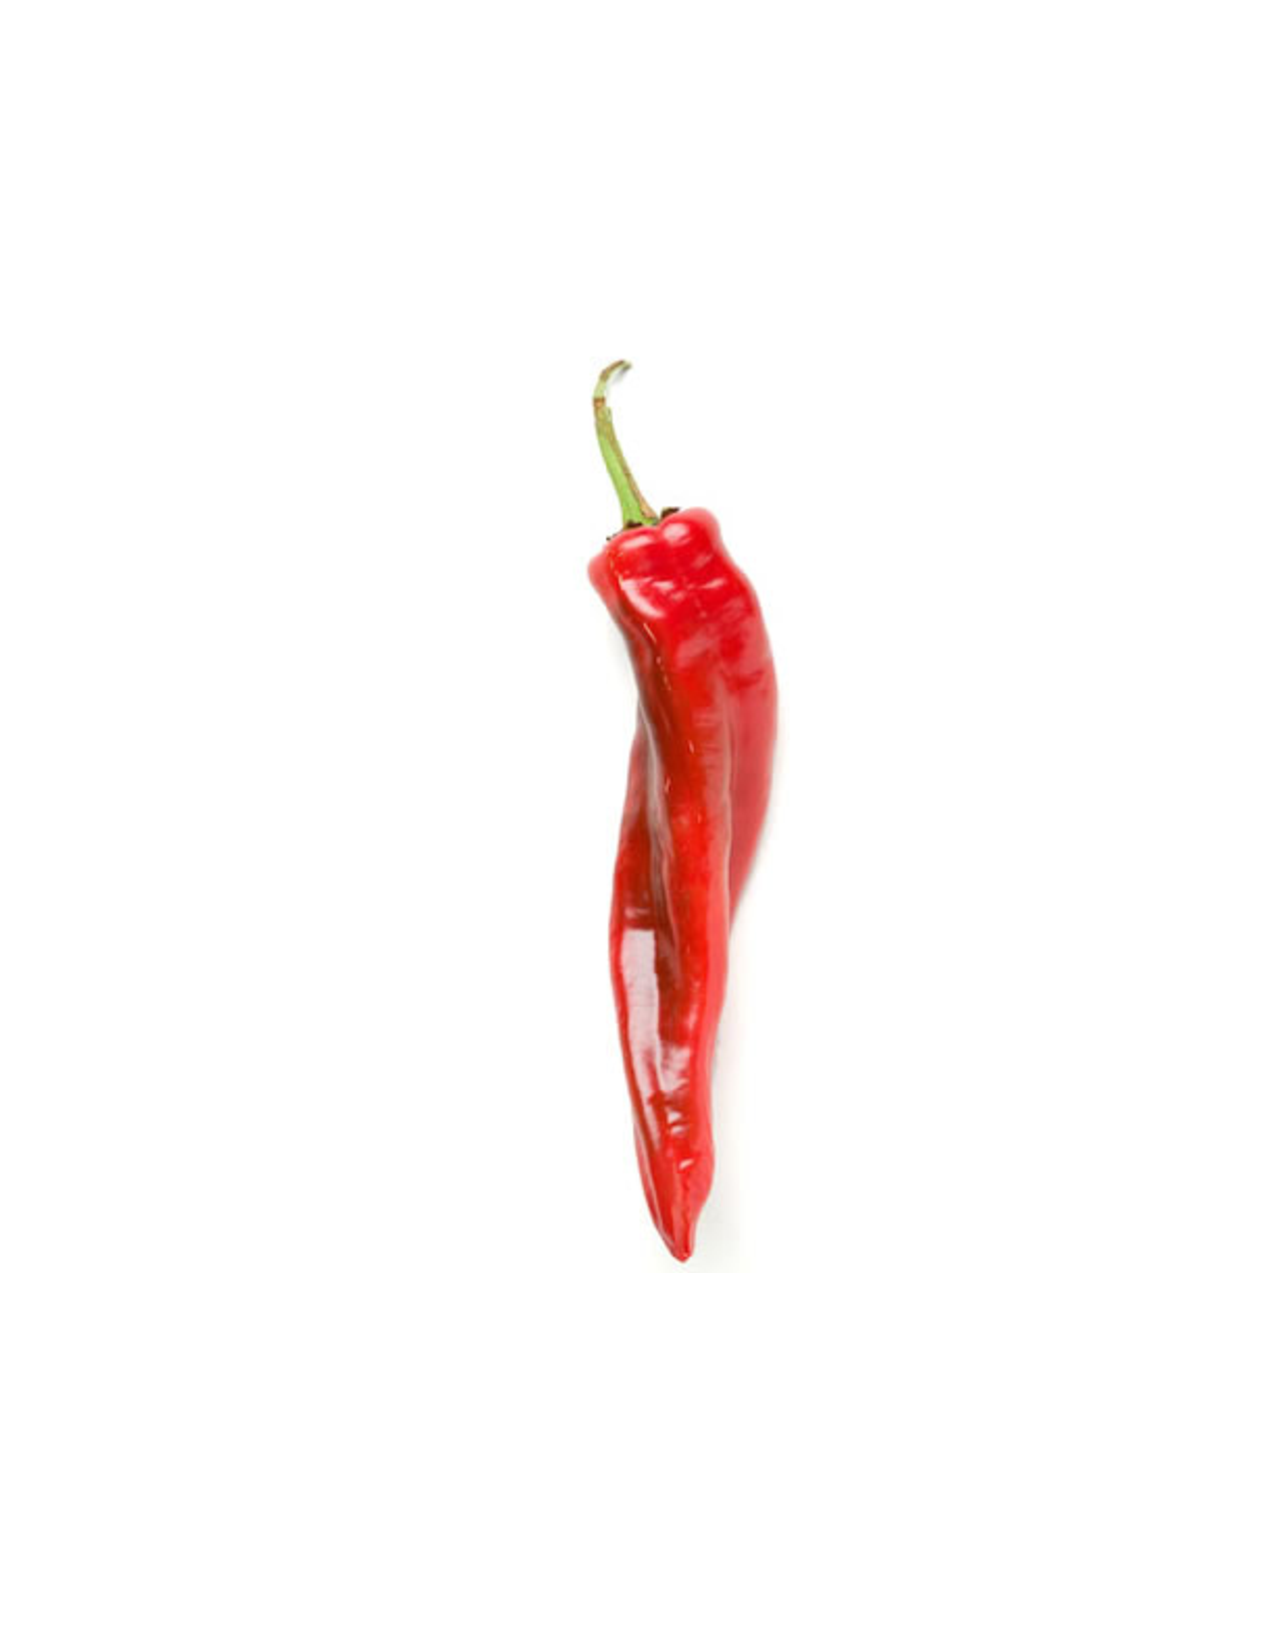
\includegraphics{figures/chili.pdf}}}
\newcommand{\chchili}{{\chili\chili}}
\newcommand{\chchchili}{{\chchili\chili}}

% The units package provides nice, non-stacked fractions and better spacing
% for units.
\usepackage{units}

% The fancyvrb package lets us customize the formatting of verbatim
% environments.  We use a slightly smaller font.
\usepackage{fancyvrb}
\fvset{fontsize=\normalsize}

% Small sections of multiple columns
\usepackage{multicol}

\hypersetup{
urlcolor=blue,
colorlinks=true
}
\usepackage[noline, procnumbered, linesnumberedhidden, boxed]{algorithm2e}

\newcommand{\openepigraph}[2]{ % This block sets up a command for printing an epigraph with 2 arguments - the quote and the author
\begin{fullwidth}
\sffamily\large
\begin{doublespace}
\noindent\allcaps{#1}\\ % The quote
\noindent\allcaps{#2} % The author
\end{doublespace}
\end{fullwidth}
}

\newcommand{\figref}[1]{Figure~\ref{#1}}
\renewcommand{\thefigure}{\arabic{figure}}

\newenvironment{callout}[1]{
\[
  \left[
      \begin{tabular}{@{\quad}m{.05\textwidth}@{\qquad}m{.75\textwidth}@{\quad}}
        \scalebox{1.5}{#1} & 
          \raggedright%
}
{
      \end{tabular}
    \right]
\]
}

\newcommand{\blankpage}{\newpage\hbox{}\thispagestyle{empty}\newpage} % Command to insert a blank page

\usepackage{makeidx} % Used to generate the index
\makeindex % Generate the index which is printed at the end of the document

\renewcommand{\maketitlepage}[0]{%
  \cleardoublepage%
  {%
  \sffamily%
  \begin{fullwidth}%
  ~
  \vspace{11.5pc}%
  \fontsize{36}{40}\selectfont\par\noindent\textcolor{darkgray}{\allcaps{\thanklesstitle}}%
  
\scalebox{.2}{
\includegraphics{figures/msan-logo}}
  \vspace{11.5pc}%
  \fontsize{12}{18}\selectfont\par\indent\textcolor{darkgray}{\allcaps{\thanklessauthor}\\
\indent{\tt parrt@cs.usfca.edu}\\
\href{http://parrt.cs.usfca.edu}{http://parrt.cs.usfca.edu}}%
  \vspace{11.5pc}%
  \fontsize{14}{16}\selectfont\par\noindent\allcaps{\thanklesspublisher}%
  \end{fullwidth}%
  }
  \thispagestyle{empty}%
  \clearpage%
}

\titlecontents{part}% FIXME
    [0em] % distance from left margin
    {\vspace{1.5\baselineskip}\begin{fullwidth}\LARGE\rmfamily\itshape} % above (global formatting of entry)
    {\contentslabel{2em}} % before w/label (label = ``II'')
    {} % before w/o label
    {\rmfamily\upshape\qquad\thecontentspage} % filler + page (leaders and page num)
    [\end{fullwidth}] % after

  \titlecontents{chapter}%
    [0em] % distance from left margin
    {\vspace{1.5\baselineskip}\begin{fullwidth}\Large\rmfamily\itshape} % above (global formatting of entry)
    {\hspace*{0em}\contentslabel{2em}} % before w/label (label = ``2'')
    {\hspace*{4em}} % before w/o label
    {\rmfamily\upshape\qquad\thecontentspage} % filler + page (leaders and page num)
    [\end{fullwidth}] % after

\titlespacing*{\chapter}{0pt}{0pt}{30pt}
\titlespacing*{\section}{0pt}{3.5ex plus 1ex minus .2ex}{2.3ex plus .2ex}
\titlespacing*{\subsection}{0pt}{3.25ex plus 1ex minus .2ex}{1.5ex plus.2ex}

\begin{document}
\chapter{Predicting Murder Rates With Gradient Descent}

\section{Goal}

\begin{fullwidth}

The goal of this project is to extend the techniques we learned in class, for one-dimensional gradient descent, to a two-dimensional domain space, solving a {\em linear regression problem}.  This problem is also known as {\em curve fitting}.  As part of this lab, you will learn how to compute with vectors instead of scalars. Please use file {\tt regression/minimize.py} for function {\tt regression/plot\_regression.py} for the code that draws the trace of the minimization in action (i.e., this is the file that has all the matplotlib junk).  You'll see starter (and test) files in the \href{https://github.com/parrt/msan501-starterkit/tree/master/regression}{\textcolor{blue}{regression starterkit}}. You will be doing your work in directory {\em userid}-{\tt regression}.

\section{Discussion}

\subsection{Problem statement}

Given training data $(x_i, y_i)$ for $i=1..n$ samples with dependent variable $y_i$, we would like to predict $y$ for some $x$'s not in our training set. $x_i$ is generally a vector of independent variables but we'll use a scalar. If we assume there is a linear relationship between $x$ and $y$, then we can draw a line through the data and predict future values with that line function. To do that, we need to compute the two parameters of our model: a slope and a $y$ intercept. (We will see the model below.)

For example, if we compare the number of murders per 100,000 people in Detroit to the average hourly wage, our eyeballs easily detect a correlation.  Here is data suitable to copy and paste into Python:

\begin{pyverbatim}
HOURLY_WAGE = [2.98, 3.09, 3.23, 3.33, 3.46, 3.6, 3.73, 2.91, 4.25, 4.47, 5.04, 5.47, 5.76]
MURDERS = [8.6, 8.9, 8.52, 8.89, 13.07, 14.57, 21.36, 28.03, 31.49, 37.39, 46.26, 47.24, 52.33]
\end{pyverbatim}

\noindent and here is a scatter plot and best fit line as determined by numpy (using {\tt\footnotesize np.polyfit(HOURLY\_WAGE, MURDERS,1)}).

\scalebox{.4}{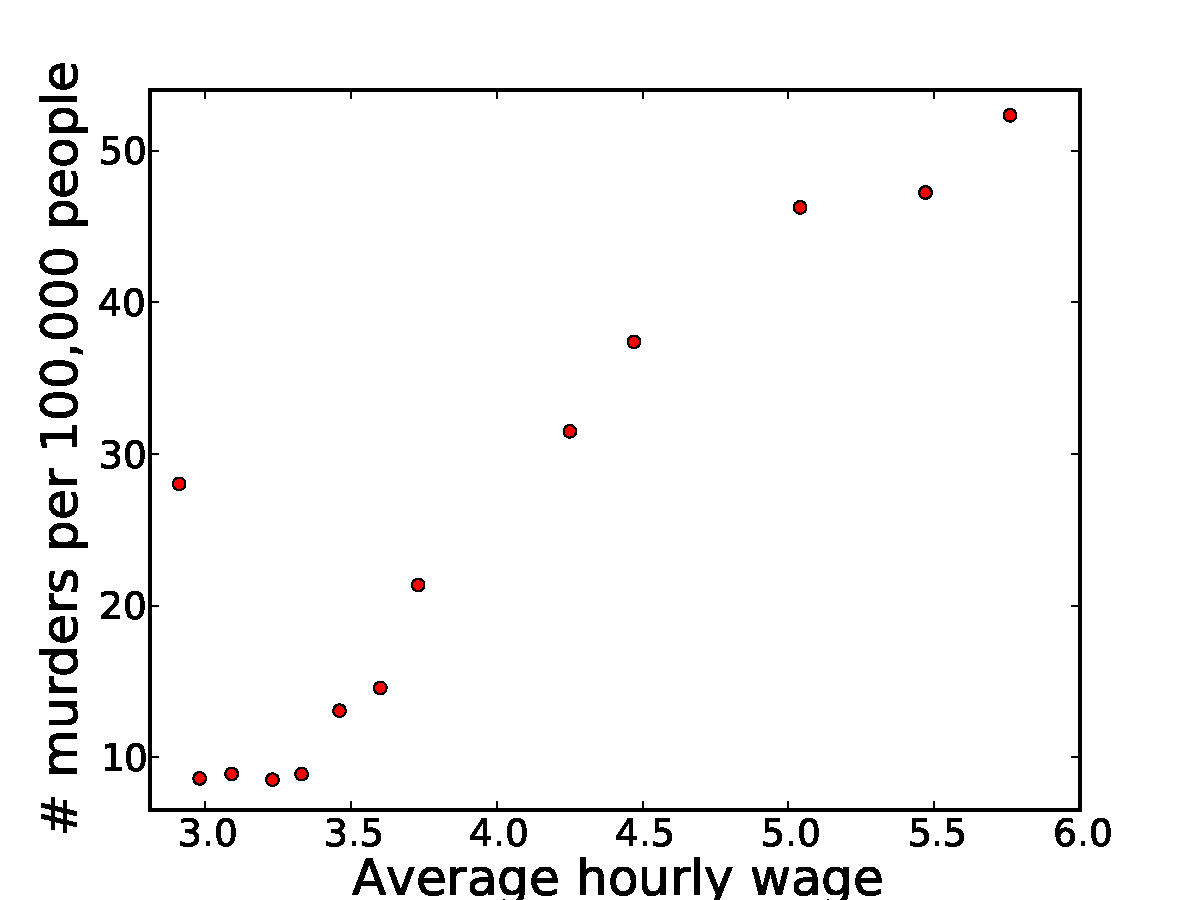
\includegraphics{figures/wage-murders.pdf}}
\scalebox{.4}{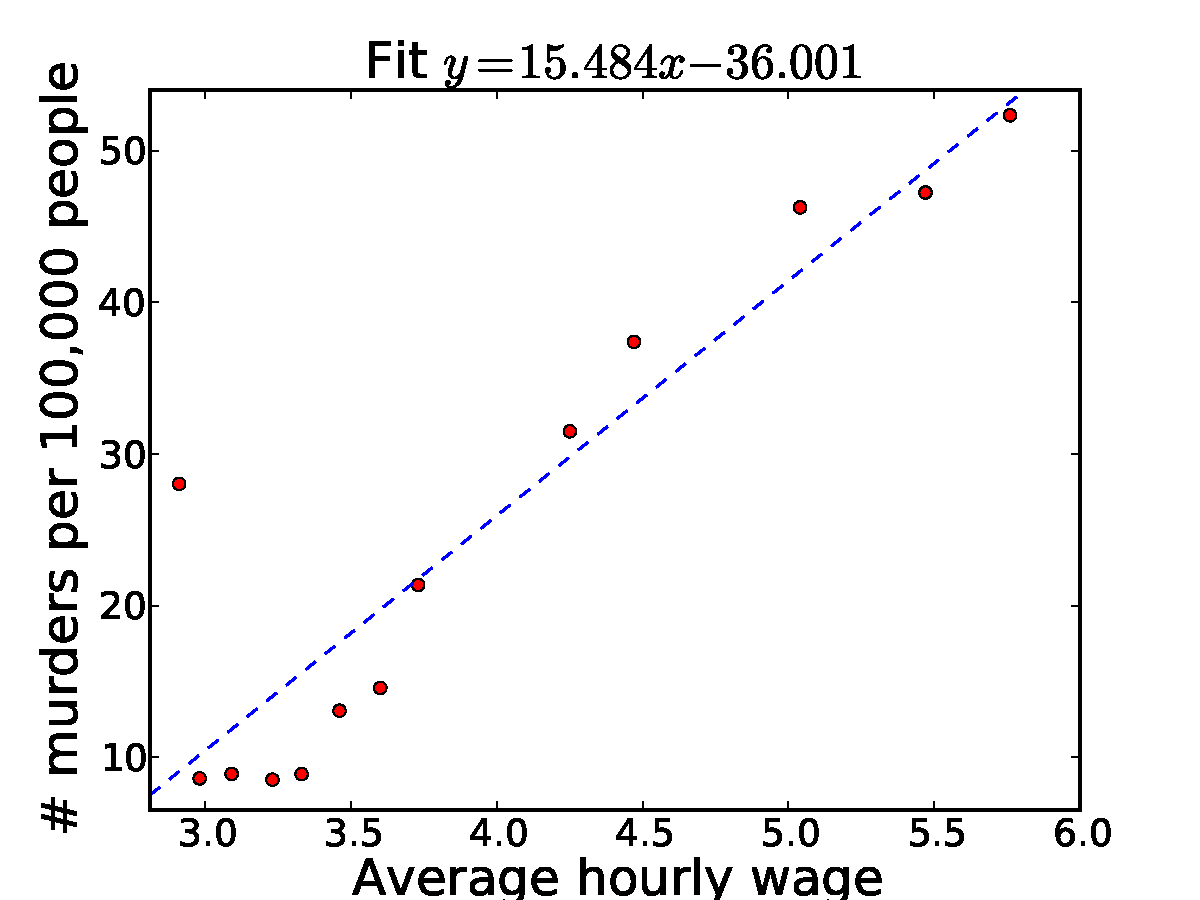
\includegraphics{figures/wage-murders-fit.pdf}}\\

\noindent Here, for example, $x_0 = 2.98$ and $y_0 = 8.6$.

{\em This might be a good point to remind everyone that correlation does not equal causation.}  I hardly think that paying people more makes them murderous, although I could see the opposite. ;)  Correlation is a {\em necessary} but not {\em sufficient} condition for causation. When you find a correlation, that gives you a candidate to check for cause-and-effect.

Here's another fun data set from {\tt\small http://www.tylervigen.com/spurious-correlations}:

\begin{pyverbatim}
# http://www.census.gov/compendia/statab/2012/tables/12s0217.xls
MOZZ_CHEESE_PER_CAPITA_2000_2009 = [9.3, 9.7, 9.7, 9.7, 9.9, 10.2, 10.5, 11.0, 10.6, 10.6]
# http://www.nsf.gov/statistics/infbrief/nsf11305/
CIVIL_ENG_PHD_2000_2009          = [480, 501, 540, 552, 547, 622, 655, 701, 712, 708]
\end{pyverbatim}

\begin{center}
\scalebox{.9}{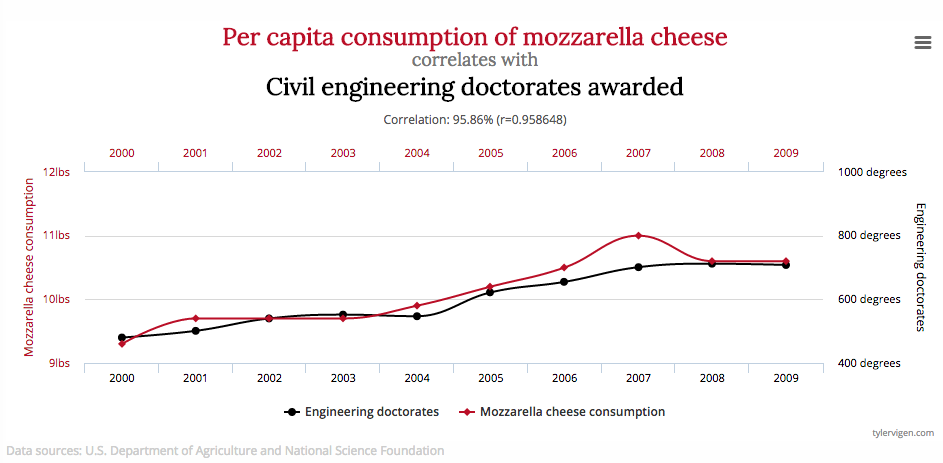
\includegraphics{figures/cheese-vs-eng.png}}
\end{center}

\subsection{Best fit line that minimizes squared error}

Recall the formula for a line from high school: $y = m x + b$.  We normally rewrite that using elements of a vector coefficients, $\vec{B}$, in preparation for describing it with vector notation from linear algebra. For simplicity,  though, we'll stick with scalar coefficients for now:

\[
\hat{y} = b_2 x + b_1
\]

\noindent We use notation $\hat{y}$ to indicate that it approximates $y$ from our data set but is not necessarily equal to any of the $y_i$.

The ``best line'' is one that minimizes some cost function that compares the known each $y_i$ value at $x_i$ to the predicted $\hat{y}$ of the linear model that we conjure up using parameters $b_1$, $b_2$. A good measure is the {\em sum of squared errors}. The cost function adds up all of these squared errors to tell us how good of a fit our linear model is:

\[
Cost(B) = \sum_{i=1}^{n}(\underbrace{\hat{y}}_\text{linear model} - \overbrace{y_i}^\text{true value})^2
\]

\noindent Inlining the expression for our model, we get:

\[
Cost(B) = \sum_{i=1}^{n}(b_2 x_i + b_1 - y_i)^2
\]

\noindent As we wiggle the linear model parameters, the value of the cost function will change.  The following graphs shows the errors/residuals that are squared and summed to get the overall cost for two different ``curve fits.''

\begin{center}
\scalebox{.35}{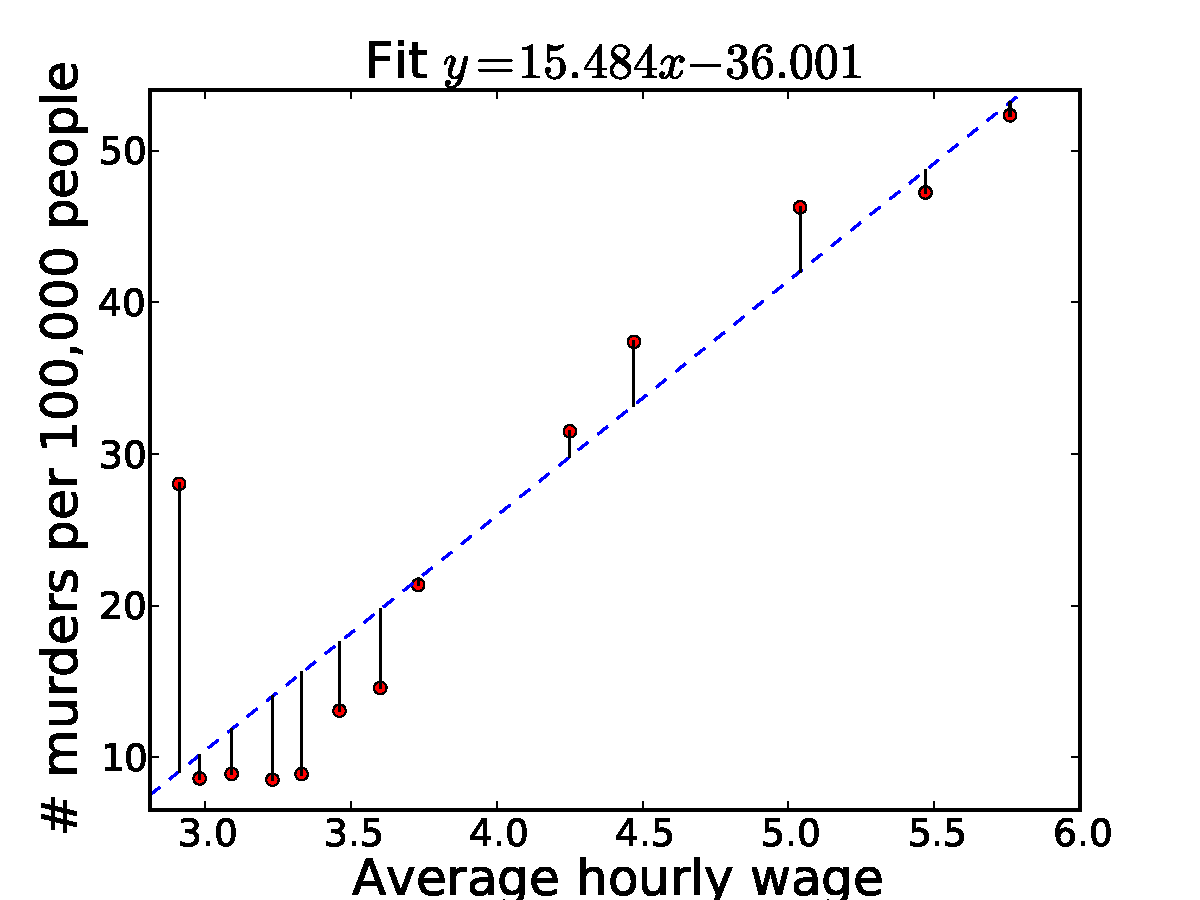
\includegraphics{figures/wage-murders-residuals.pdf}}
\scalebox{.35}{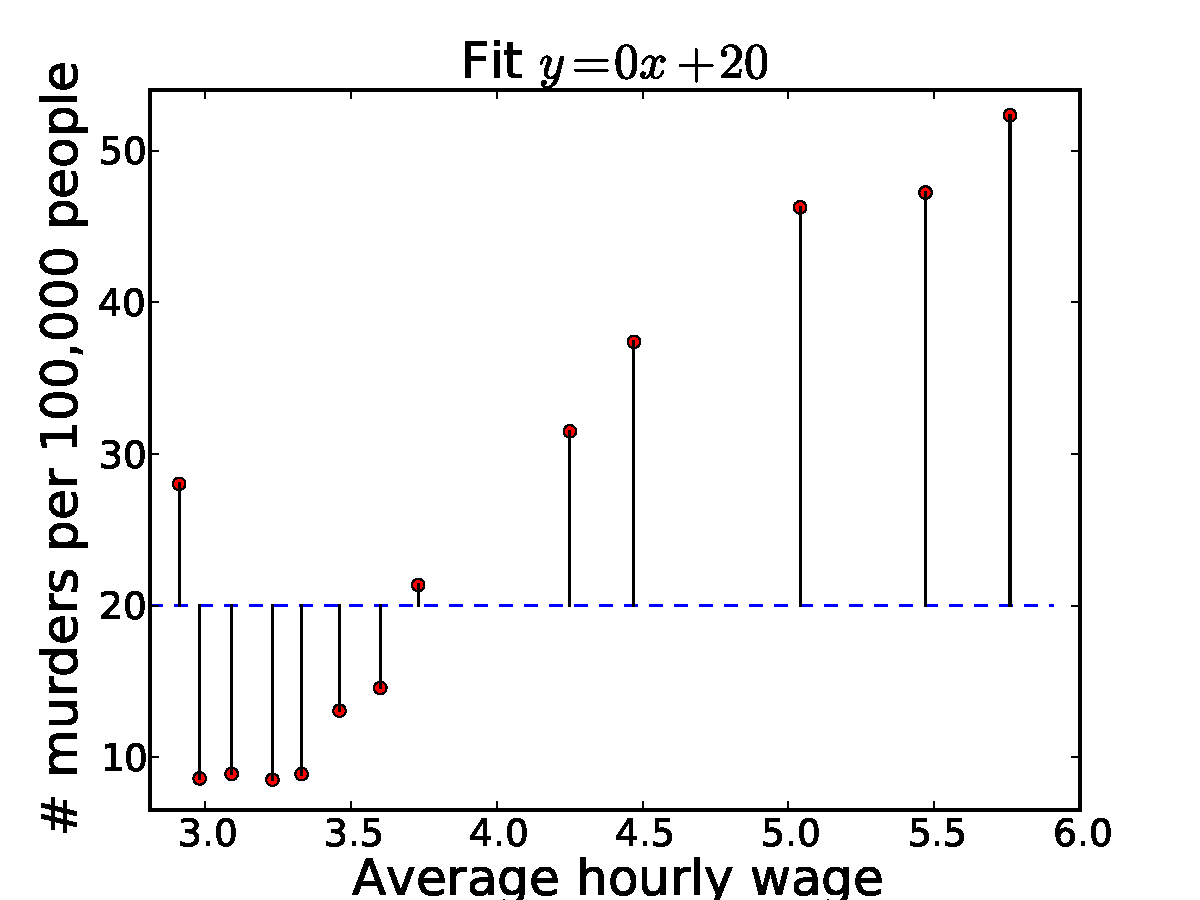
\includegraphics{figures/wage-murders-residuals-poor.pdf}}\\
\end{center}

\noindent The costs are 533.82 for the left and 3563.50 for the right.

The good news is that we know the cost function is a quadratic (by construction), which is convex and has an exact solution. All we have to do is figure out where the cost function flattens out. Mathematically, that is when the partial derivatives of the cost function are both zero. The partial derivative for a particular dimension is just the rate of change of that dimension at a particular spot. It's like a skier examining the slope of her skis against the mountain one at a time.
\[\tag{Analytic solution to optimization}
\nabla Cost(B) = 0
\]

\noindent For our purposes, though, we'll use gradient descent to minimize the cost function. There are lots and lots of cost functions that are not simple little quadratics with symbolic solutions from calculus. In those cases, we have to use computer simulation.

To show our prediction model in action, we can ask how many murders  there would be in Detroit if the average wage were \$4.7? (Obviously, these wages are from 30 years ago.) To make a prediction, all we have to do is plug $x=4.7$ into $\hat{y} = 14.484 x - 36.001$, which gives us 32.074 murders.

\subsection{Gradient descent in 3D}

Before trying to minimize the cost function, it's helpful to study what the surface looks like in three dimensions, as shown in the following two graphs. The X and Y dimensions are the coefficients of our linear model and the Z coordinate (up) is the cost function.

\noindent \scalebox{.45}{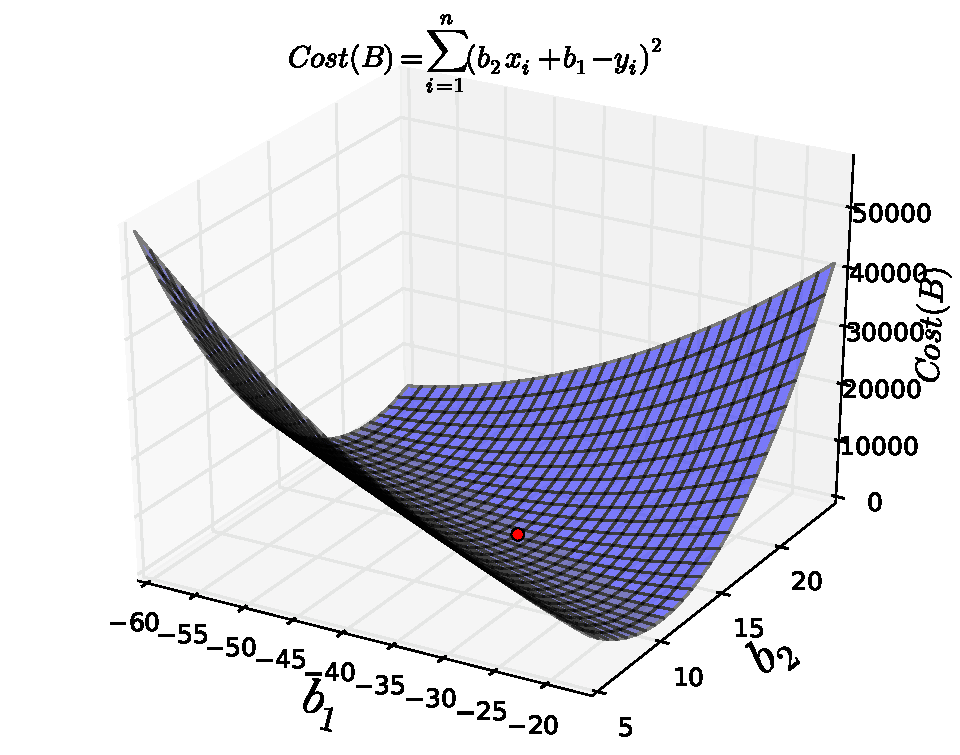
\includegraphics{figures/wage-murders-cost-3d.pdf}}
\scalebox{.45}{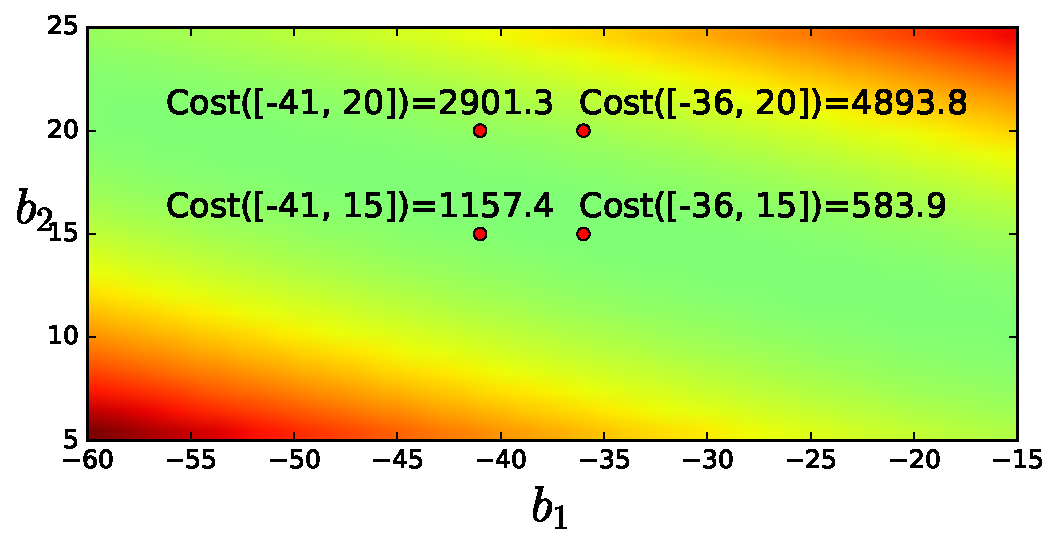
\includegraphics{figures/wage-murders-heatmap.pdf}}

What surprised me is that changes to the slope of the linear model's coefficient $b_2$, away from the optimal $b_2=15.484$, cost much more than tweaks to the y intercept, $b_1$. Regardless, the surface is convex. Unfortunately, based upon the deep trough that grows slowly along the diagonal of $(b_1,b_2)$, gradient descent takes a while to converge to the minimum. We will examine the path of gradient descent for a few initial starting point. Wikipedia says that the Rosenbrock function is a pathological case for traditional gradient descent and it looks pretty similar to our surface with its shallow valley in this topographic view from above:

\scalebox{.4}{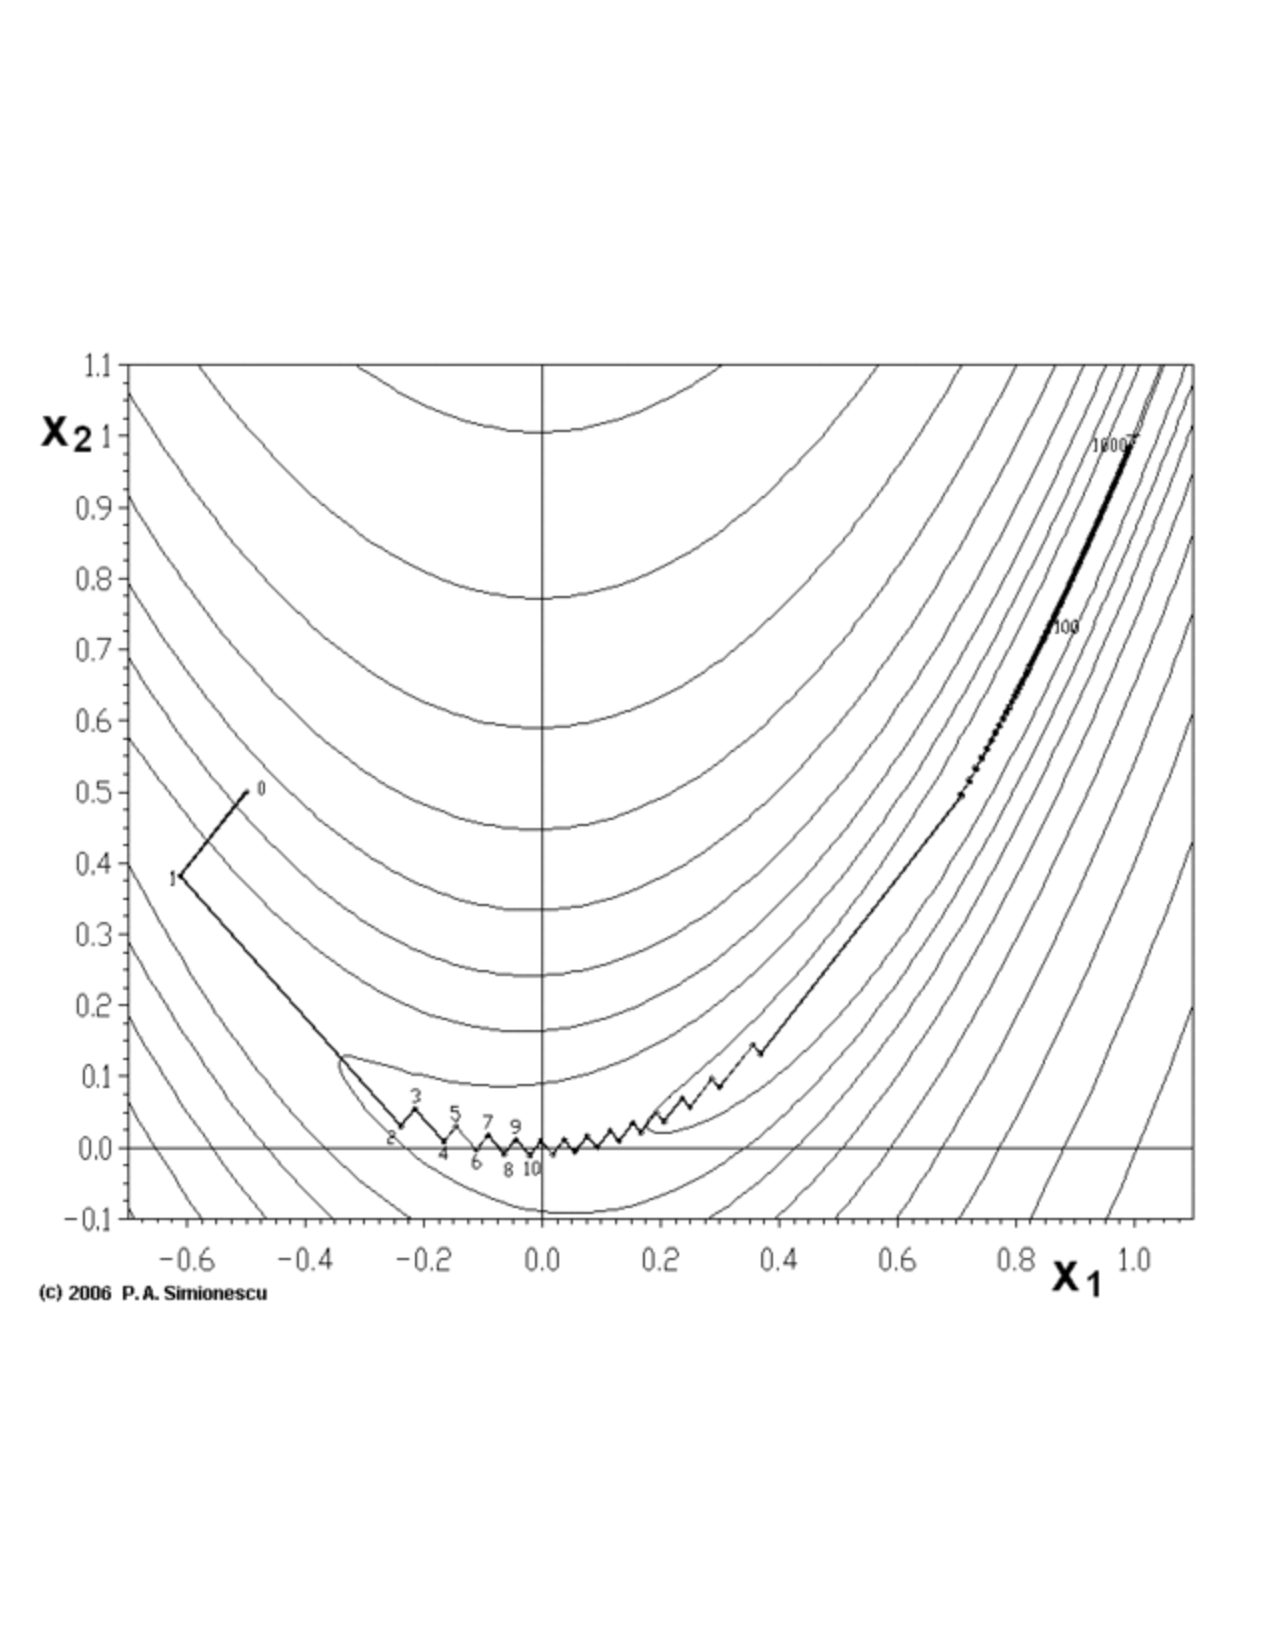
\includegraphics{figures/Banana-SteepDesc}}

The recurrence relation for updating our estimate of $\vec{B}=[b_1, b_2]$ that minimizes $Cost(\vec{B})$ is the same as the single-variable gradient-descent we did in class but with a vector instead of a scalar:

\[
\vec{B}_{i+1} = \vec{B}_i - \eta \nabla Cost(\vec{B}_i)
\]

\noindent where we will approximate vectors of partial derivatives with partial finite differences:

\[
\nabla F(\vec{X}) =
\begin{bmatrix}
\frac{\partial}{x_1}{F(\vec{X})}\\
\frac{\partial}{x_2}{F(\vec{X})} \\
\end{bmatrix}
\approx
\begin{bmatrix}
\frac{F(\left[ x_1+h \above 0pt{x_2} \right]) - F(\vec{X})}{h} \\
\frac{F(\left[ x_1 \above 0pt{x_2+h} \right]) - F(\vec{X})}{h} \\
\end{bmatrix}
\]

\noindent The $h$ variable is a very small delta step away from a specific coordinate in each dimension in turn. In our case, we will compute the components of a finite difference vector $C'$ ignoring the division by the step $h$ because it will get folded into our learning rate $\eta$.

\subsection{Gradient-descent algorithm}

The minimization algorithm looks like:

\begin{enumerate}
\item Pick an initial $B_0$
\item Let $B = B_0$
\item $C' = \left[ Cost(\left[ b_1+h \above 0pt{b_2} \right]) - Cost(B_i) \above 0pt Cost(\left[ b_1 \above 0pt{b_2+h} \right]) - Cost(B_i) \right]$, the finite difference in each direction computed separately
\item Let $B_{i+1} = B_i - \eta C'$
\item Goto step 3 until $abs(Cost(B_{i+1})-Cost(B_i)) < precision$ {\bf and} when the $Cost$ starts going back up
\end{enumerate}

Using a small learning rate, my solution takes 4843 steps starting from coordinate (-45,10) using a very small step size, which gives me a fairly decent approximation of the minimum: [-36.00066933  15.48414587] compared to the analytic solution [ -36.000625 15.484375 ]. Starting from about the same distance away in the shallow valley at (-45,25), my solution takes 5142 steps. Cutting my step size by 5x, takes 30463 steps but gives a slightly more precise result [-36.00063497  15.48432944]. Starting at (-45,25) takes 31958 steps. Surprisingly, when I start very close to the minimum at (-36,15), my solution takes 47350 steps and does not exactly give a more accurate result. ``{\em Your mileage may vary.}''

\noindent \scalebox{.45}{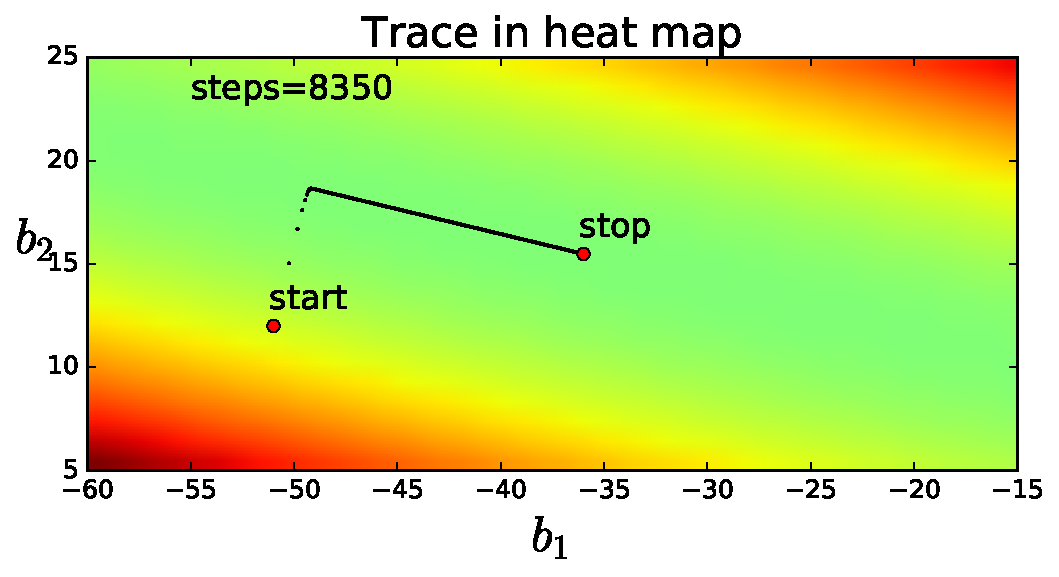
\includegraphics{figures/wage-murders-heatmap-trace1.pdf}}
\scalebox{.45}{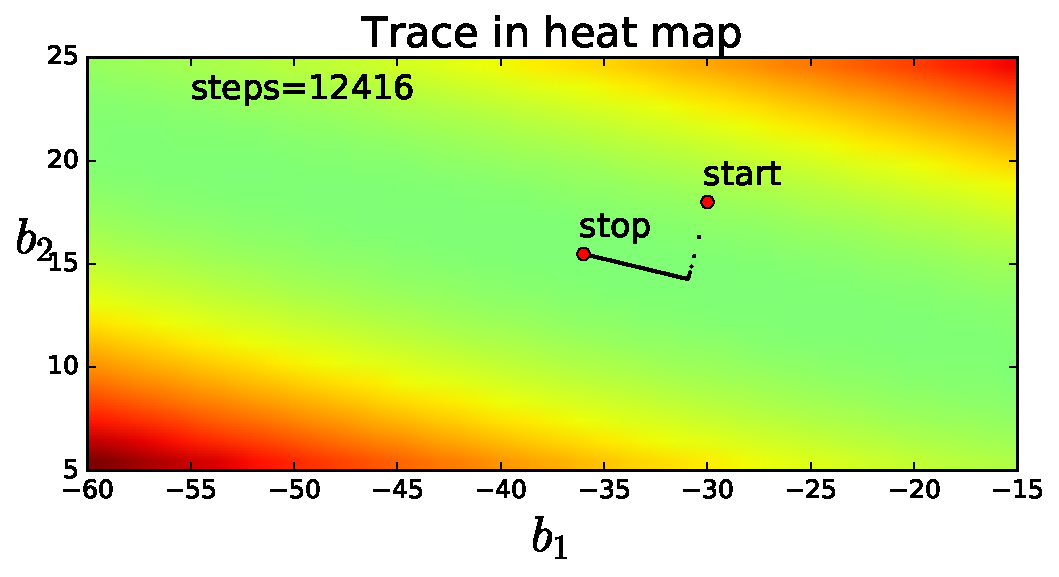
\includegraphics{figures/wage-murders-heatmap-trace2.pdf}}

\noindent \scalebox{.45}{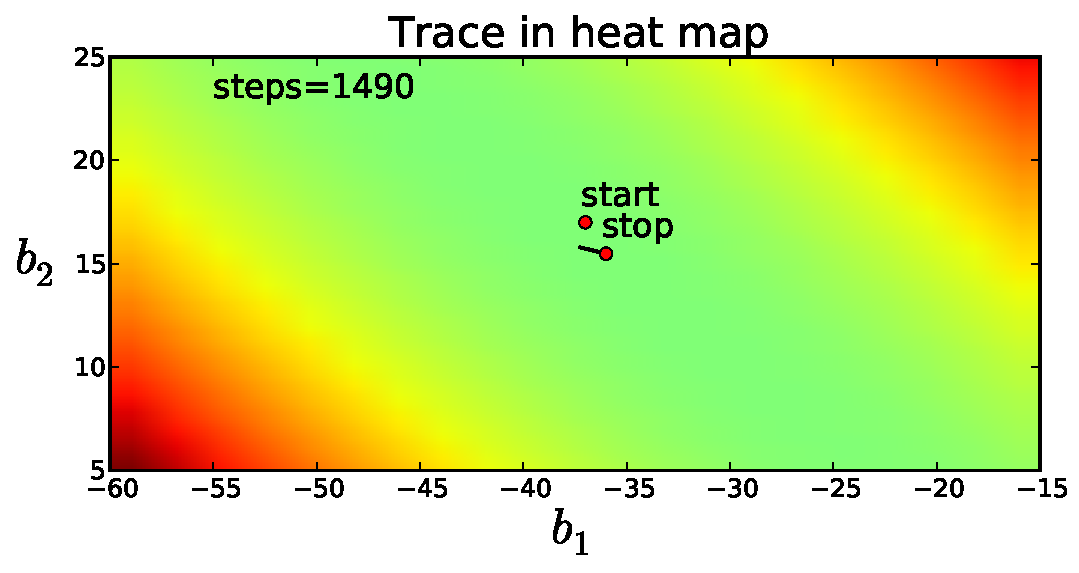
\includegraphics{figures/wage-murders-heatmap-trace3.pdf}}

When I crank up the learning rate and use a very small step size, my solution converges must faster and with the same accuracy. For example, with 10 times the learning rate as before, (-45,25) converges in 3193 steps instead of 31958 steps.

\section{Getting fancy}

For the most part, the algorithm described above converges on the analytic solution with a high degree of precision, assuming that your $h$ is small enough. In some cases however it only gets 3 digits of precision versus about six, depending on where the starting point is. To improve that accuracy, we can improve our termination condition from simply comparing previous and new value of the cost function to use the Euclidean distance between $B_{i+1}$ and $B_i$ or the magnitude of the finite difference. 

To increase convergence rate, it's a good idea to have different $\eta$ learning rates per dimension, particularly in this case because we want to speed along the valley of $b_1$, but not jump too far on $b_2$ as it is already steep; the finite difference will cause it to move along quickly. {\em Note:} Because numpy will overload the {\tt *} multiple operator to work with vectors as well as scalars, $\eta$ can be a 2-vector and $\eta C'$ will ``just work.''

For extremely large data sets or very high dimension data sets, you can use {\em stochastic gradient descent} which takes a single random or a small random subset of the samples when computing the cost function. Surprisingly, this still converges and takes much less time to compute. I believe that the math says that the algorithm will converge no matter how many samples (don't quote me on that). Further, picking a random subset adds noise to the process, which has been shown to pull gradient descent out of local minima and get it moving again towards a lower minimum. In our case, there is an exact solution and therefore a single minimum so we would only get a speed benefit from stochastic gradient descent.

\section{Your task}

You will use gradient descent to solve the linear regression problem above, using the same data. As part of your final submission, you must provide heat maps with traces that indicate the steps taken by your gradient descent as I have shown above.  Have your program choose two random starting $B_0$ vectors (you can use {\tt random.randrange()}) to produce your heat maps.   In {\tt regression/minimize.py}, define a function called {\tt minimize} that takes the indicated parameters and returns the minimum $B$ parameters of your linear model, the number of steps, and the trace array of intermediate $B_i$ values ($B$ is a list of 2-vectors).

\begin{pyverbatim}
def minimize(f, B0, eta, h, precision):
    trace = []
    B = B0
    steps = 0 
    while True:
        steps += 1
        if steps % 10 == 0: # only capture every 10th value
            trace.append(B)
        ...     
    ... 
    return (B, steps, trace)
\end{pyverbatim}

\noindent As an example, in my {\tt regression/plot\_regression.py} script, I call that function like this:

\begin{pyverbatim}
(m,steps,trace) = minimize(Cost, B0, LEARNING_RATE, h, PRECISION)
\end{pyverbatim}

Use {\tt pylab.imshow()} to draw the heat map whose $b_1$ are the $y$ intercepts, $b_2$ coordinates are the slopes, and heat value is the cost of $x,y$.  Hide all of your heat map construction in function in {\tt regression/plot\_regression.py}:

\begin{pyverbatim}
def heatmap(X, Y, f, trace=None): # trace is a list of [b1, b2] pairs
    ...
\end{pyverbatim}

\noindent so we can call it like this:

\begin{pyverbatim}
heatmap(HOURLY_WAGE, MURDERS, Cost, trace)
plt.show() # finally show the heatmap
\end{pyverbatim}

Your {\tt heatmap} function will create two ranges for the $b_1$ and $b_2$ coordinates and then simply compute the cost,  storing it in a matrix such as {\tt C[b1][b2] = Cost([b1,b2],...)}.  The trace is plotted on top of the map once you create it. The coordinate ranges of the heat map are not related to the trace at all. It took me a while to figure out all of the crazy methods to draw the heat maps so I'll toss you a bone and just provide it for you (it goes in your {\tt heatmap()} function):

\begin{pyverbatim}
	imshow(C,
		   origin='lower',
		   extent=[min(b1), max(b1), min(b2), max(b2)],
		   vmax=abs(C).max(), vmin=-abs(C).max()
	)
\end{pyverbatim}

\noindent I plot the trace using:

\begin{pyverbatim}
plt.plot(p[0], p[1], "ko", markersize=1)
\end{pyverbatim}

Please show the information as I have shown in the graphs to make it easier to compare results and for me to grade. 

You will have to pick an appropriately small step value $h$ to get a decent approximation of the derivative through finite differences. You want that number to be small enough that your algorithm does not oscillate around the minimum. If the number is too big it will compute a finite difference that leads to $B_{i+1}$ leaping across the minimum to the other wall of the function. You must pick a learning rate $\eta$ that allows you to go as fast as you can but not so fast that it overruns the minimum back and forth. When I crank up my learning rate too far, I also see the algorithm go off into the weeds and stops with a minimum of [ -4.86000929e+10  -2.85744570e+12].

\section{Testing}

You can run {\tt regression/test\_regression.py} to check your {\tt miminize} function.  Here's my sample run:

\begin{lstlisting}[style=BashInputStyle]
$ python test_regression.py
starting at [-23, 12]
gradient descent gives  [-36.00034331  15.48430239] Cost 533.815093809
exact is                [-36.000625000000007, 15.484375]
starting at [-50, 10]
gradient descent gives  [-36.00062579  15.48437039] Cost 533.815093755
exact is                [-36.000625000000007, 15.484375]
starting at [-36, 17]
gradient descent gives  [-36.00062582  15.4843704 ] Cost 533.815093755
exact is                [-36.000625000000007, 15.484375]
starting at [-36, 15]
gradient descent gives  [-36.00034331  15.48430239] Cost 533.815093809
exact is                [-36.000625000000007, 15.484375]
starting at [100, 17]
gradient descent gives  [-36.00034316  15.48430235] Cost 533.815093809
exact is                [-36.000625000000007, 15.484375]
starting at [-15, 0]
gradient descent gives  [-36.00034325  15.48430237] Cost 533.815093809
exact is                [-36.000625000000007, 15.484375]
\end{lstlisting}

\section{Resources}

There is a lot of material out there on the web that can be helpful.

\begin{itemize}
\item \href{http://en.wikipedia.org/wiki/Finite_difference}{Finite difference at Wikipedia}
\item \href{http://research.microsoft.com/pubs/192769/tricks-2012.pdf}{Stochastic Gradient Descent Tricks}
\item \href{http://apps.nrbook.com/fortran/index.html}{Numerical recipes (See Chap 10 on minimization of functions)}
\item \href{http://adl.stanford.edu/aa222/Lecture_Notes_files/AA222-Lecture2.pdf}{Single verbal minimization in line searches}
\item \href{http://cs229.stanford.edu/notes/cs229-notes1.pdf}{Andrew Ng's CS229 Lecture notes}
\item \href{http://people.duke.edu/~ccc14/pcfb/analysis.html}{Data analysis with Python}
\end{itemize}

{\bf You must tweak the step size and other parameters so that your results agree with the first {\bf three} decimal points of the analytic solution [-36.000625000000007, 15.484375].} (My solution is much better than that, except for a couple of weird starting positions where it only gets three decimal places.)

\begin{callout}{\bcplume}
\begin{itemize}
\item Your script {\tt regression/minimize.py} with the {\tt minimize()} function.
\item Your script {\tt regression/plot\_regression.py}, which must have your {\tt heatmap} function.  This file imports the previous.
\item A PDF of your graph with two visible traces on two heat maps or the same heat map if the traces are clear. The graph should include the start, stop location and the number of steps as I have done on mine. As part of your PDF, please indicate the $B$ parameters you compute with your minimize function.
\end{itemize}
\end{callout}

\end{fullwidth}

\end{document}